\chapter{Contextual Analysis}
During the contextual analysis phase the abstract syntax tree (AST) is traversed to check the semantics of the given program. This means both the  scope rules and type rules need to be checked for validity, and they will be defined in this following section.

\section{Abstract syntax trees}\label{ca:ast}
% Chapter 7 Fischer 
The AST is a data structure designed to be used in all activities after the syntactic analysis. This is done in order to spread functionality in the compiler to different components to increase maintainability and make it more understandable. The abstract syntax tree is similar to a parse tree, but has certain unnecessary details omitted. The AST consists of nodes. These nodes can be parents, children or siblings in relation to which node is currently being examined \cite{CraftinfACompiler}.
\\\\
To make an efficient AST structure, it should account for the following:
\begin{itemize}
    \item ASTs are typically constructed bottom-up, and should support tree construction from the leaves toward the root.
    \item The list of siblings is generated through recursive rules.
    \item Some nodes have a fixed number of children, and some can require a random amount. An example of a node requiring a fixed amount of children would be the addition operation, requiring two numbers to add together. An example of a node requiring a different amount of nodes would be a list, as the user defines how many elements they want the list to contain.
\end{itemize}
%Taking these considerations into account, each node in the tree has certain pointers to be able to traverse the tree effectively:
%\begin{itemize}
%    \item Each node points to the next sibling, and to its leftmost sibling.
 %    \item Each node points to its leftmost child.
%    \item Each node points to its parent.
%\end{itemize} \todo{Gør vi faktisk det her i vores AST?????????????!??!?}
\subsubsection{Design of the AST}
Since the AST is involved in most compiler phases, certain characteristics should be emphasised in the final design.

\begin{itemize}
    \item There should be enough information to unparse the AST, meaning the program should be able to be reconstructed.
    \item The implementation should be separated from the essential information within the AST to facilitate use in each of the compiler's phases.
    \item The different phases of the compiler will view the AST differently.
\end{itemize}
Finally, for reference we include a picture of a regular concrete parse tree and the AST for the same input. These can be seen on \ref{fig:syntax-AST}.

\begin{figure}[H]
\centering
  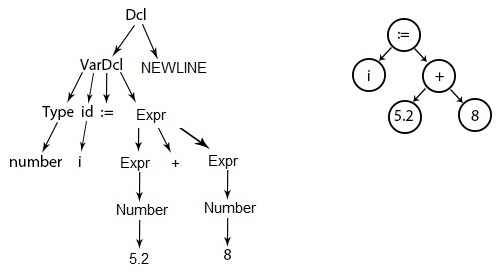
\includegraphics[width=0.8\textwidth]{figures/Syntax-AST.jpg}
  \caption{This figure shows the syntax tree (left) and AST (right) for the syntax \textit{number i := 5.2 + 8}.}
  \label{fig:syntax-AST}
\end{figure}


\section{Scope rules}
The scope rules of PHAL tell us which bindings are in effect under the execution of procedures. 
There are two kinds of scope rules which are dynamic and static.
Dynamic scope rules use bindings that are in effect when the procedure is called. 
This means that the scope is determined at run time.
\\\\
Static scope rules only use the bindings that where in effect when the procedure was declared. 
So the scope can already be determined at compile time.
We choose to use static scope rules in PHAL. 
The reasoning behind this is that we deemed static scope rules to be simplest to work with for the programmer. 
Static scope rules are also the most common scope rules for programming languages \cite{PilenVedTraeetsRod}. 
This means that if the programmer has any experience in programming then static scope rules will most likely be the most intuitive for them to work with. 
\\\\
For the functions in PHAL, we wish to have call-by-value, which means that when a variable is passed as an argument for a function, it is a copy of the variable's value that is parsed to the function.
\\\\
As described in the MoSCoW for PHAL, Section~\ref{section:moscow}, the implementation of a reference parameter will be considered, but not necessarily implemented. 
This allows the user to use pass by reference instead of pass by value.


\section{Formal definition}\label{Def:Semantics}
Once the informal definition of PHAL has been created, a formal definition needs to be formulated in order to remove any doubt about the behaviour of the language. 

\subsection{Syntactic categories}
The syntactic categories define the fundamental constructs of the language, and the elements in each category are represented by metavariables. These metavariables are defined in Table~\ref{tab:syntacticcategories}, and are used to ensure that it is clear when for example \textit{x, n, gx} or \textit{a} are variables that are already defined with a specific contextual meaning. Metavariables are different to regular variables. Regular variables could be defined as for example $y$, $z$, $obj$ or any other combination not present in the syntactic categories \cite{PilenVedTraeetsRod}. If multiple metavariables from the same category are present in a rule, they will be indexed - for example if two boolean expressions $b$ appear, they will be written as $b_1$ and $b_2$ respectively. 
\begin{table}[H]
\centering
\begin{tabular}{@{}lll@{}}
\toprule
Variable &       & Description                      \\ \midrule
$n$        & $\in$ & \textbf{Num} - Number                     \\
$x$        & $\in$ & \textbf{Var} - Variable                     \\
$gx$        & $\in$ & \textbf{GVar} - A variable of the group type                     \\
$lx$        & $\in$ & \textbf{LVar} - A variable of the list type                     \\
$\epsilon$ & $\in$ & \textbf{Epsilon} - The empty string \\
$new$      & $\in$ &  \textbf{Newl} - Newline                   \\
$a$        & $\in$ & \textbf{Aexp} - Arithmetic expression                    \\
$b$        & $\in$ & \textbf{Bexp} - Boolean expression                    \\
$adt$        & $\in$ & \textbf{Adv} - Advanced data type                     \\
$f$       & $\in$ & \textbf{FuncName} - The name of a function      \\
$S$        & $\in$ & \textbf{Stmt} - Statements               \\
$D_V$       & $\in$ & \textbf{VarDcl} - Declaration of a variable \\
$D_G$       & $\in$ & \textbf{GroupDcl} - Declaration of a group \\
$D_L$       & $\in$ & \textbf{ListDcl} - Declaration of a list \\
$D_F$       & $\in$ & \textbf{FuncDcl} - Declaration of a function \\
$D_{Adt}$       & $\in$ & \textbf{AdvDcl} - Declaration of an advanced type      \\
$D_P$       & $\in$ & \textbf{ParamDcl} - Declaration of parameters for a function \\
$P$       & $\in$ & \textbf{ParamOpt} - The parameter options \\
$Pin$      & $\in$ &  \textbf{Pins} - The pins that are used to connect the Arduino \\
$RTN$       & $\in$ & \textbf{Rtrn} - The returntypes \\
$P_S$        & $\in$ & \textbf{ProgStart} - The start of the program \\
$S_B$       & $\in$ & \textbf{SetBody} - The construction of setup      \\
$G_B$       & $\in$ & \textbf{GrpBody} - The body of the group \\
$L_B$       & $\in$ & \textbf{ListBody} - The body of the list \\
$L_T$       & $\in$ & \textbf{ListType} - The type of the list \\
$F_B$      & $\in$ &  \textbf{FuncBody} - The user defined function body  \\ 
$F_N$      & $\in$ &  \textbf{FuncNames} - The function names  \\
$L_N$      & $\in$ &  \textbf{ListNames} - The list names  \\
$G_N$      & $\in$ &  \textbf{GrpNames} - The group names  \\\bottomrule
\end{tabular}
\caption{Syntactic categories of PHAL}
\label{tab:syntacticcategories}
\end{table}
\noindent
These categories are necessary as we will be using the defined metavariable names within to construct an abstract syntax for PHAL.


\subsubsection{Abstract syntax for PHAL}
The abstract syntax describes the linguistic constructions of the language.
For every syntactic category the structure of the elements are described through a collection of construction rules, given in the form of context free production rules. 
These rules are seen for the categories in Table~\ref{tab:syntacticcategories}, with the exception of numbers $n$, variables $x$ and $newl$, because these are assumed to respectively be numerals, a collection of characters and the terminating character for lines in PHAL. 
Numerals in the context of semantics are defined as syntactic descriptions of numbers, so not actual numbers, but rather words for the numbers \cite{PilenVedTraeetsRod}. 
The category \textit{Epsilon} will only be detailed through rules in relation to a certain category of the abstract syntax. 
This category is the one concerning declarations, and it will be detailed in Section~\ref{subsec:declarations}.

\begin{table}[H]
\centering
\begin{tabular}{@{}lll@{}}
\toprule
Variable &       & Description                      \\ \midrule
$a$        & $::=$ & $n$ | $x$ | $gx$ | $lx$ | $a_1 + a_2$ | $a_1 - a_2$ | $a_1 * a_2$ | $a_1 \div a_2$ | $a_1 \bmod a_2$ | $ (a_1) $    \\
$b$        & $::=$ & $a_1 = a_2$ | $a_1 != a_2$ | $a_1 > a_2$ | $a_1 < a_2$ | $a_1 <= a_2$ | $a_1 >= a_2$            \\
            & & | $!b$ | $b_1$ \& $b_2$ | $b_1 | b_2$ | $(b_1)$  \\
            &&  | $a_1$ is $a_2$ | $b_1$ and $b_2$  | $b_1$ or $b_2$ |  $a_1$ is not $a_2$ | not $b$ \\
            &&  | $a_1$ greater than $a_2$  |  $a_1$ less than $a_2$  | $a_1$ less than or equal to $a_2$  \\
            &&  | $a_1$ greater than or equal to $a_2$ \\
            & & | true | false | on | off \\
$P_S$      & $::=$ & setup $S_B$ repeat $S$ $D_F$\\
$S_B$    & $::=$ & $S_B$ \textit{new} $S_B$ | $Dv$ | $D_G$ | $D_L$ | $D_{adt}$ | $S$\\ 
$S$        & $::=$ & $x:= a$ | $x:= b$ | $x \text{ += } x$ | $x \text{ += } a$ | $x \text{ -= } x$  \\
           & & | $x \text{ -= } a$ | $gx := b$ | $S_1 \textit{new} \: S_2$ | if $b$ then $S$ $S_{if}$ | if $b$ then $S$ \\
           & & | loop $S$ until $b$ | loop $S$ until $b$ increase $x$ by $n$  \\
           & & | loop $S$ until $b$ decrease $x$ by $n$ | loop $S$ $a$ times \\
           & & |  call $f$ with $y...y_n$ | call $f$ with $a...a_n$  \\
           & & | switch($a|b$) case $<a_1|b_1>: \: S_1$ $...$ case $<a_n|b_n>: \: S_n$ default: $S$ \\
           &&  | get element $n$ from $lx$ | remove element $n$ from $lx$  \\
           &&  | add $a$ to $lx$ | add $b$ to $lx$ | $\text{wait for } a \text{ seconds}$  \\
$S_{if}$     & $::=$ &  else if $b$ then \{$S$\} | else if $b$ then \{$S$\} $S_{if}$ |  else \{$S$\} \\
$D_V$       & $::=$ & $var$ $x := a \: \textit{new}$ $D_V$ | $var$ $x := b \: \textit{new}$ $D_V$ | $\epsilon$ \\
$D_G$       & $::=$ & group $gx$ $G_B$ \textit{new} $D_G$ \\
$G_B$      & $::=$ & adt x \textit{new} $G_B$ | group gx \textit{new} $G_B$ | $\epsilon$ \\
$D_L$     & $::=$ &  list $L_T$ $lx$ $L_B$ \textit{new} $D_L$ \\
$L_T $     & $::=$ &  group | number | bool | text | motor | temperatureSensor | lightbulb\\
$L_B $     & $::=$ &  $a$, $L_B$ | $x$, $L_B$ | $gx, \: L_B$ | $b, \: L_B$ | $a$ | $x$ | $gx$ | $b$ | $\epsilon$ \\
$D_F$       & $::=$ & define $f$ with $P$ $F_B \: \text{returnType} \: RTN \: \textit{new}$ $D_F$ | $\epsilon$ \\
$P$ & $::=$ & none | $D_P$ \\
$D_P$  & $::=$ & var x, $D_P$ | group gx, $D_P$ | adt x, $D_P$ | list lx, $D_P$ | var x \\
            & & | group gx | adt x | list lx  \\  
$RTN$       & $:=$ &  none | number | text | bool | group | list | adt\\
$F_B$       & $:=$ &  $F_B$ \textit{new} $F_B$| $D_V$ | $D_P$ | $D_G$ | $D_L$ | $S$ | $S_{wait}$ | return $x$\\
$D_{Adt}$   & $::=$ & $adt$ $x$ $:=$ pin $Pin \: new \: D_{adt} | \: \epsilon  $  \\ 
$adt$   & $::=$ & motor | temperatureSensor | lightbulb     \\ 
$Pin$       & $::=$ & $ n, Pin$ | $n$ \\
\bottomrule
\end{tabular}
\caption{Abstract syntax of PHAL}
\label{tab:syntacticformation}
\end{table}
\noindent 
\subsection{Environment-store-model}\label{semantics:EnvStore}
In order to formally define the semantic rules for PHAL we will construct big-step-operational semantic rules for the language. 
This will be done through the \textit{environment-store-model}. This model is used to describe how variables are bound to values through what is called a \textit{variable environment} and a \textit{storage}. 
Variables are bound to a location address, and each location address is bound to a value. 
This value is then the value of the variable that points to that location. 
As such, the \textit{environment-store-model} describes both the locations in memory and which values are stored there.
A visual representation of the model can be seen on Figure~\ref{fig:ESModel}.
\\\\
The variable-environment is essentially a symbol table containing the variable and the address. 
The \textit{storage} describes which values are found at the different storage locations, by defining the value and storage connection \cite{PilenVedTraeetsRod}. 
The values stored in storage can either be numbers, text, booleans or advanced data types.
\\
Figure~\ref{fig:ESModel} gives an illustration of this, where the variables describe a location, and the location describes the storage. 
The variable table contains a \textit{next} variable, that points to the next unused location. 
\begin{figure}[H]
\centering
  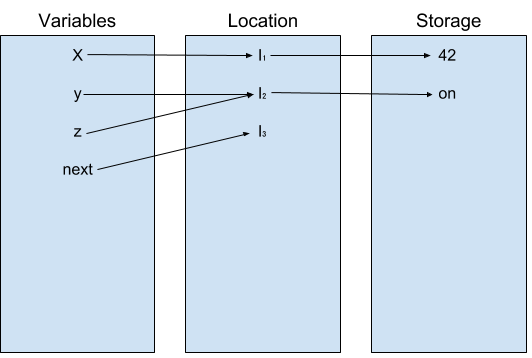
\includegraphics[width=0.7\textwidth]{figures/semantics/1.png}
  \caption{This figure shows an example of the Environment-Store Model.}
  \label{fig:ESModel}
\end{figure}


\noindent
The set of variable-environments is the set of partial functions from the variables to the locations, denoted $EnvV$. 
A single element of $EnvV$ is defined as $env_v$. $EnvV$ is defined as such:
\begin{equation*}
\centering
    EnvV = Var \cup next \rightharpoonup Loc
\end{equation*}
This means the variable environment is a list of variables and a next variable that all point to a location.
\\\\
 The set of possible storage locations is denoted $Loc$. Locations are assumed to be of the set of integers, as this is satisfactory for the purposes with which the model will be used in this section. This means the locations are defined as \\ 
\begin{equation*}
\centering
    Loc = \mathbb{Z}
\end{equation*}
\\
The set of storage values is the set of partial functions from location to values, defined as:
\begin{equation*}
Sto = Loc \rightharpoonup Number \cup Text \cup Bool \cup Adt
\end{equation*}
This means that each element in the list of locations point to a value in storage that is typed as either a number, text or bool. 
A single element of $Sto$ is defined as $sto$. 
\\\\
These sets are defined through partial functions because it is not necessary to explain the location of every single variable imaginable, but rather just the ones that are used.

\subsection{Transition systems}
Defining operational semantics is done by defining a transition system. The transition system is an oriented graph, where the edges are equivalent to a step of a program and the vertices represent a snapshot of the program \cite{PilenVedTraeetsRod}. In operational semantics, the edges are called transition and the vertices are called configurations. Vertices without outgoing edges are called the ending configurations. The transition system is then defined as the following triple:
\\
\begin{equation*}
\centering
    (\Gamma, \xrightarrow{}, T)
\end{equation*}
$\Gamma$ is a set of configurations, $\xrightarrow{}$ is the transition relation and $T$ is a subset of $\Gamma$, denoting the ending configurations.
To further illustrate, a finite transition system is shown in the following figure:
\begin{figure}[H]
\centering
  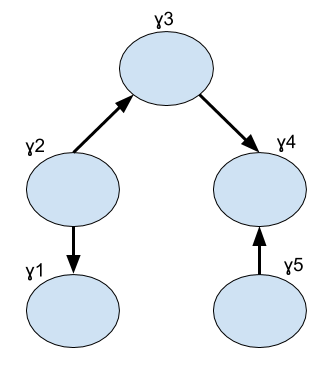
\includegraphics[width=0.4\textwidth]{figures/semantics/TransistionssystemsFigur.png}
  \caption{An example of a transition system}
  \label{fig:TransistionSystem}
\end{figure}
\noindent
On Figure~\ref{fig:TransistionSystem}, the possible configurations $\Gamma$ is the set $\{\gamma1, \gamma2, \gamma3, \gamma4 \text{ and } \gamma5\}$. The transition relation is given through pairs $(\gamma, \gamma')$, denoting that there is a transition from $\gamma$ to $\gamma'$. For the example, the transition relation is then: 
\begin{center}
$\xrightarrow{} \: = \{(\gamma2, \gamma1),\: (\gamma2, \gamma3), \:(\gamma3, \gamma4), \:(\gamma5, \gamma4)\}$
\end{center}
The ending configurations have no outgoing transitions, and thus for the example the set $\{\gamma1, \: \gamma4\}$ makes up the ending configurations $T$.

\subsection{Reading structural operational semantic rules}
Big step semantic rules are constructed using premises, conclusions and side conditions. 
The general shape of a rule is that, given one or more environments and a store, the premises of the rule specifies how the conclusion reaches the result of modified environments and a modified store.
\\\\
In addition to the premise and conclusion, the rule can make use of a side conditions to define for which cases the conclusion holds. An example of the setup of a rule would be like this:
\begin{equation}\label{EQ:exampleSemantic}
\cfrac
{
    environment, \: store \vdash \: Premise \xrightarrow{} updated \: env \: and \: sto
}
{ 
    environment, \: store \vdash Conclusion \xrightarrow{} updated \: env \: and \: sto
}
\quad side \: condition
\end{equation}
The $\vdash$ operator shown before the premise and the conclusion describes what knowledge you need to properly define the rule. 
So for this example, in order to reach the conclusion, knowledge of both the current environment and the current store would be necessary. 
An introductory example constructed for PHAL, including all the elements of a semantic rule, would be the rule for adding numbers together as shown on Equation~\ref{EQ:SemainticsArithmeticExprPLUSNumber}
\begin{equation}\label{EQ:SemainticsArithmeticExprPLUSNumber}
\begin{minipage}{.2\linewidth}
$[\text{PLUS-num}_\text{BSS}]$
\end{minipage}
\begin{minipage}{.8\linewidth}
\centering
$\cfrac{env_v, \: sto \vdash a_1 \xrightarrow{}\textsubscript{a} \: v_1 \quad env_v, \: sto \vdash a_2 \xrightarrow{}\textsubscript{a} \: v_2}{env_v, \: sto \vdash a_1 + a_2 \xrightarrow{}\textsubscript{a} \: v}$
$ \: where$ $v$ $=$ $v_1$ $+$ $v_2$
\end{minipage}
\end{equation}
The semantic rule shown on Equation~\ref{EQ:SemainticsArithmeticExprPLUSNumber} looks similar to Equation~\ref{EQ:exampleSemantic}, with the main difference being the premises. 
There are multiple premises in the PLUS rule, and they do not lead to an updated environment or store. 
This is common for rules concerning expressions, whereas the one explicitly shown on Equation~\ref{EQ:exampleSemantic} is more common for statements and declarations. 
This is due to expressions by themselves not affecting the environments or storages - in the case of PLUS, it merely computes the value of the addition of the two numbers. 
Declarations update environments because they save information about a declaration, meaning the environment containing that declaration will be different after the execution of the declaration. Statements change values based on context, meaning they can cause changes in the values in storage, thereby updating it.
\\\\
Equation~\ref{EQ:SemainticsArithmeticExprPLUSNumber} states that when the variable environment and storage are known, the statement $a_1 + a_2$ can be evaluated to a value $v$ if $a_1$ can be evaluated to a value $v_1$, and $a_2$ can be evaluated to a value $v_2$, when they meet the requirement specified in the side condition that states that $v = v_1 + v_2$. 
The arrows that appear in both the premises and the conclusion indicate that the evaluation of these values must be done through the transition relation for arithmetic expressions. 
This means that they must be evaluable through one of the transitions defined for arithmetic expressions. The full list of these is contained in Appendix~\ref{AppSec:SemainticsArithmeticExpr}.
\\

\subsection{Semantic rules of PHAL}
Using the big step semantic rules described, the semantic rules of PHAL can be described.
\subsubsection{Arithmetic expressions}\label{sem:aexp}
In the following subsection a small selection of the semantic rules for arithmetic expressions is shown and described, the full list can be seen in Appendix~\ref{AppSec:SemainticsArithmeticExpr}. 
The semantic rules for arithmetic expressions are based on the transition system 
\begin{equation*}
(\textbf{Aexp} \cup \; \mathbb{Q}, \: \xrightarrow{}\textsubscript{a}, \: \mathbb{Q})    
\end{equation*}
In the system, the possible configurations $\Gamma$ are given as all the possible expressions given by \textbf{Aexp} defined by the metavariable $a$ in the syntactic categories in Table~ \ref{tab:syntacticformation}, the transition relations $\xrightarrow{}\textsubscript{a}$ are given by the rules defined in Appendix~\ref{AppSec:SemainticsArithmeticExpr}, and the ending configurations $T$ are a subset of all possible configurations.
\\\\ 
In this case $T$ is given as the final value of an arithmetic expression $\mathbb{Q}$, as they are values and have no outgoing transitions.

\begin{equation}\label{EQ:SemainticsArithmeticExprPLUSText}
\begin{minipage}{.2\linewidth}
$[\text{PLUS-text}_\text{BSS}]$
\end{minipage}
\begin{minipage}{.8\linewidth}
\centering
$\cfrac{env_v, \: sto \vdash a_1 \xrightarrow{}\textsubscript{a} \: v_1 \: \: \: env_v, \: sto \vdash a_2 \xrightarrow{}\textsubscript{a} \: v_2}{env_v, \: sto \vdash a_1 + a_2 \xrightarrow{}\textsubscript{a} \: v}$
$ \: where$ $v$ $=$ $v_1$ $\circ$ $v_2$
\end{minipage}
\end{equation}
On Equation~\ref{EQ:SemainticsArithmeticExprPLUSText} the semantic rule for concatenating two strings can be seen. The rule states that when the variable environment and storage are known, the statement $a_1 + a_2$ can be evaluated to a value $v$, but only if $a_1$ can be evaluated to a value $v_1$ and $a_2$ can be evaluated to a value $v_2$, and the value of $v$ is the value of $v_1 \circ v_2$, as specified in the side condition.
\\\\
For the next rule, a function to convert from the syntactic description of numbers as numerals to actual numbers. This function is defined as:
\begin{equation*}
    \mathcal{N}: Num \xrightarrow{} \mathbb{Q}
\end{equation*}
$\mathbb{Q}$ denotes the set of rational numbers, meaning it allows for both integer values and decimal point values of numbers.
\begin{equation}\label{EQ:numbss}
\begin{minipage}{.2\linewidth}
$[\text{NUM}_\text{BSS}]$
\end{minipage}
\begin{minipage}{.8\linewidth}
\centering
$env_v, \: sto \vdash n \xrightarrow{}\textsubscript{a} \: v$ $ \: \text{if}$ $\mathcal{N}[\![n]\!]$ $=$ $v$ 
\end{minipage}
\end{equation}
The semantic rule shown on Equation~\ref{EQ:numbss} shows how a number is evaluated to an actual value from its syntactic representation. The rule states that when the variable environment and storage is known, a number $n$ can be evaluated to a value $v$ through use of the function $\mathcal{N}$.
\\
\begin{equation}\label{EQ:SemainticsArithmeticExprVAR}
\begin{minipage}{.2\linewidth}
$[\text{VAR}_\text{BSS}]$
\end{minipage}
\begin{minipage}{.8\linewidth}
\centering
$env_v, \: sto \vdash x \xrightarrow{}\textsubscript{a} \: v$ $ \quad \text{if} \quad env_v \: x = l$ and $sto \: l = v$ 
\end{minipage}
\end{equation}
On Equation \ref{EQ:SemainticsArithmeticExprVAR} the rule for evaluating variables is shown. The rule states that when the variable environment and storage is known, a variable $x$ can be evaluated to a value $v$, if the terms of the side conditions $env_v \: x = l \quad \text{and} \quad sto \: l = v$ are met. This means that the variable environment points $x$ to a location, and that the storage of that location $l$ points to the value $v$. First the location is found, and then the value contained in that location is determined.



\subsubsection{Boolean expressions}
In the following section a small selection of the semantic rules for boolean expressions is shown and described, for the full set of semantic rules see Section~\ref{AppSec:SemainticsBooleanExpr}.
Boolean expressions evaluate to either true or false, written as $tt$ and $ff$ respectively. The transition system for boolean expressions, \textit{Bexp}, is thus:
\begin{equation*}
    (\textbf{Bexp} \cup \{tt, ff\}, \xrightarrow{} \textsubscript{b}, \{tt, ff\})
\end{equation*}
The transition relation $\xrightarrow{}\textsubscript{b}$ is defined in Appendix~ \ref{AppSec:SemainticsBooleanExpr}. Some of the rules for boolean expressions require the evaluation of arithmetic expressions, and to do this the transition relation $\xrightarrow{}\textsubscript{a}$ is used as defined in Subsection~\ref{sem:aexp}.

\begin{equation}\label{EQ:SemanticsBooleanExprEQUALS}
\begin{minipage}{.2\linewidth}
$[\text{EQUALS-1}_\text{BSS}]$
\end{minipage}
\begin{minipage}{.8\linewidth}
\centering
$\cfrac{env_v, \: sto \vdash a_1 \xrightarrow{}\textsubscript{a} \: v_1 \quad\: env_v, \: sto \vdash a_2 \xrightarrow{}\textsubscript{a} \: v_2}{env_v, \: sto \vdash a_1 = a_2 \xrightarrow{}\textsubscript{b} \: tt}$
$ \: if$ $v_1$ $=$ $v_2$
\end{minipage}
\end{equation}
On Equation~\ref{EQ:SemanticsBooleanExprEQUALS} the rule for evaluating logical equals can be seen. The rule specifies that knowing the variable environment and the storage, the expression $a_1 = a_2$ can be evaluated to $tt$ if $a_1$ and $a_2$ can evaluate to values $v_1$ and $v_2$ through the transition relation $\xrightarrow{} \textsubscript{a}$, and the side condition of the rule is met. The side condition simply specifies the stipulation that the two values must be the same for the conclusion to be reached.

\begin{equation}\label{EQ:SemanticsBooleanExprGTR}
\begin{minipage}{.2\linewidth}
$[\text{GTR-1}_\text{BSS}]$
\end{minipage}
\begin{minipage}{.8\linewidth}
\centering
$\cfrac{env_v, \: sto \vdash a_1 \xrightarrow{}\textsubscript{a} \: v_1 \quad\: env_v, \: sto \vdash a_2 \xrightarrow{}\textsubscript{a} \: v_2}{env_v, \: sto \vdash a_2 > a_1 \xrightarrow{}\textsubscript{b} \: tt}$
$ \: if$ $v_2$ $>$ $v_1$
\end{minipage}
\end{equation}
The semantic rule shown on Equation~\ref{EQ:SemanticsBooleanExprGTR} describes the logical greater than operation. The rule states that when the variable environment and the storage are known, the expression $a_2 > a_1$ will evaluate to the boolean value $tt$ if both the variables $a_1$ and $a_2$ can evaluate to a value through the transition relation $\xrightarrow{} \textsubscript{a}$, and the side condition is met - being that $a_2$ has evaluated to a value that is greater than the value $a_1$ has evaluated to.
\begin{equation}\label{EQ:SemanticsBooleanExprAND}
\begin{minipage}{.2\linewidth}
$[\text{AND-1}_\text{BSS}]$
\end{minipage}
\begin{minipage}{.8\linewidth}
\centering
$\cfrac{env_v, \: sto \vdash b_1 \xrightarrow{}\textsubscript{b} \: tt \quad\: env_v, \: sto \vdash b_2 \xrightarrow{}\textsubscript{b} \: tt}{env_v, \: sto \vdash b_1 \wedge b_2 \xrightarrow{}\textsubscript{b} \: tt}$
\end{minipage}
\end{equation}
On Equation~\ref{EQ:SemanticsBooleanExprAND} the semantic rule for the logical \textit{and} operation can be seen. The rule states that, knowing the variable environment and the storage, the expression $b_1 \And b_2$ will be evaluated to true, if the values of $b_1$ and $b_2$ are both evaluated to true.




\subsection*{Declarations}\label{subsec:declarations}
PHAL has different declarations in the form of \textit{functions, variables, groups, advanced data types} and \textit{lists}. 
To facilitate the use of these different possible declarations for the differing types allowed in PHAL, it is necessary to expand the environment store model. 
The model is expanded with new environments for the types that can contain multiple instances of another type - \textit{lists} and \textit{groups}, so it is possible to keep track of which variables they contain. 
\textit{Advanced data types} are seen as a subset of variables and as such will be contained within the variable environment.
\\\\
The \textit{group} type contains a set of variables, and allows the user to assign a boolean expression to the whole group, in order to toggle the status of all the group members. 
To do this, the group must point to a location, such that this location can point to the boolean value that is assigned to the group. 
This requires further changes to the model. As defined in the previous subsection, Subsection~\ref{semantics:EnvStore}, the next pointer is currently placed in the variable environment. 
If we were to add a next pointer to the group environment, insert a group-variable into the group environment, assign it to a location and update the next pointer, it would result in a situation as depicted on Figure~\ref{fig:ESModelProblem}.
\begin{figure}[H]
\centering
  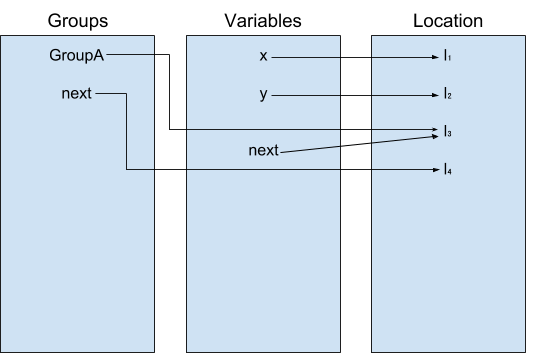
\includegraphics[width=0.7\textwidth]{figures/semantics/5.png}
  \caption{This figure illustrates the next pointer problem}
  \label{fig:ESModelProblem}
\end{figure}
\noindent
As seen on Figure~\ref{fig:ESModelProblem}, the situation where the next pointer in the group environment is updated leaves the next pointer in the variable environment pointing to a location that is already used.
\\\\
To remedy this, we either have to update both next pointers every time either environment is given a new variable, or the next pointer can be moved to storage. The solution employed is the one where the next pointer is moved to storage, as it is the most intuitive.
\\\\
This requires us to redefine the definitions from Subsection~\ref{semantics:EnvStore}. First we redefine the variable environment, as the next pointer has been removed:
\begin{center}
$EnvV = Var \rightharpoonup Loc$
\end{center}
Now the storage is redefined:
\begin{center}
$Sto = Loc \cup \text{\{next\}} \rightharpoonup Number \cup Text \cup Bool \cup Adt \cup Loc $
\end{center}
This states that $Sto$ is a partial function from either a location or the next pointer, that returns either one of the types or a location. The type will be returned if the location is given as input, and likewise the location of the next pointer will be returned when it is given as input.
\subsubsection{Variable declarations}
To declare variables we must define the operational semantics for the \textit{VarDcl} category. 
Variable declarations modify both the storage and the variable environment, due to binding new locations to variables and assigning values to these locations. This gives us the transition relation $\xrightarrow{}\textsubscript{Dv}$ and the system ($\Gamma \textsubscript{Dv}, \xrightarrow{}\textsubscript{Dv}, T \textsubscript{Dv}$). The configurations are defined as:
\\
The possible configurations are $\Gamma \textsubscript{Dv} = (VarDcl \times EnvV \times Sto) \cup EnvV \times Sto$\\
The ending configurations are
$T\textsubscript{Dv} = EnvV \times Sto$ meaning that all variable declarations must point to either a variable or a place in the storage. 
\\\\
As such, the transition takes the shape $\langle D_V, \: env_V, \: sto \rangle \xrightarrow{}\textsubscript{Dv} (env'_v, \: sto')$ In order to construct the semantic rules, we introduce the function $new: Loc \xrightarrow{} Loc$. This function returns the next possible location for any given location. As locations are of the type integer, this is defined as $new l = l + 1$.

\begin{equation}\label{rule:vardcl}
\begin{minipage}{.2\linewidth}
$[\text{AVARDCL}_\text{BSS}]$
\end{minipage}
\begin{minipage}{.8\linewidth}
\centering
$\cfrac{\langle Dv, \: env_v [x \mapsto l], \: sto[l \mapsto v] \: [next \mapsto new \: l]\rangle \xrightarrow{}\textsubscript{Dv} \: (env_v', sto') }{\langle var \: x:= a \: \textit{newline} \: Dv, \: env_v, \: sto \rangle \xrightarrow{}\textsubscript{Dv} \: (env_v', sto')}$
\[where \: env_v, \: sto \vdash a \xrightarrow{}\textsubscript{a} \: v \: and \: l = sto \: \text{next}\]
\end{minipage}
\end{equation}
The rule~\ref{rule:vardcl} shows that we bind $x$ to $l$ where $l$ is the next free location as specified in the side condition. After this, the $next$ pointer is bound to a newly created location after $l$ using the $new$ function.

\subsubsection{Group declarations}
Groups in PHAL are defined in Section~\ref{sec:phalvsarduino}. To relate this to the environment store model, the Figures~\ref{fig:emptyGroup} and \ref{fig:groupA} have been constructed to aid the explanation. 

\begin{figure}[H]
\centering
  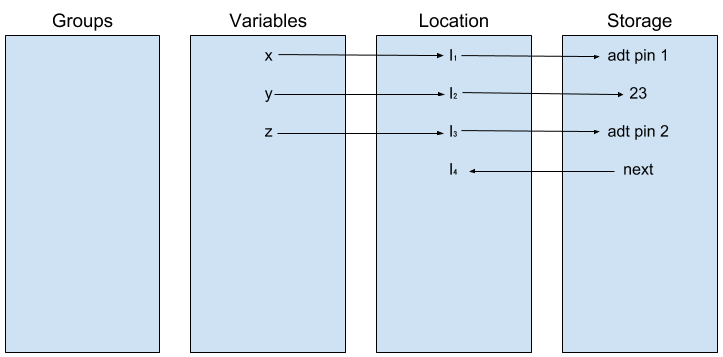
\includegraphics[width=10cm]{figures/semantics/2.png}
  \caption{The expanded model prior to declaration}
  \label{fig:emptyGroup}
\end{figure}
\noindent
Figure~\ref{fig:emptyGroup} shows a visualisation of the environment store model with the added group environment prior to declaring a group. The figure simply illustrates that the functionality of the model is kept intact - variables bind to a location, locations bind to a storage and the next pointer points to the next free location from storage.
\begin{figure}[H]
\centering
  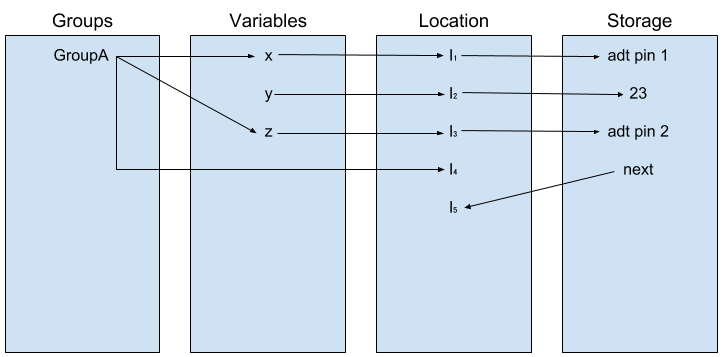
\includegraphics[width=10cm]{figures/semantics/3.png}
  \caption{The expanded model after declaration}
  \label{fig:groupA}
\end{figure}
\noindent
This figure shows the needed functionality for the model when a group has been declared. In order to keep track of the variables contained in the group, we define the \textit{group environment} $EnvG$. This environment is similar to the one defined for variables in Section~\ref{semantics:EnvStore}, but contains bindings from groups to variables rather than variables to location. In order to facilitate a group assignment statement to change the value of all elements of the group, it is also necessary to assign the group to a location during the declaration. Finally, we allow a recursive definition of groups, meaning a group can contain other groups. This gives the following definition:
\\
\begin{center}
$EnvG = GrpNames \rightharpoonup \mathcal{P}(EnvV) \times Loc \times \mathcal{P}(EnvG)$
\end{center}
A single element from $EnvG$ is defined as $env_G$. 
The definition is based on groups only allowing advanced data type variables in their body, as per the definition in Subsection~\ref{Def:Types} and no functions or declarations of any type. The definition  states that for every group name the partial function will return the variables from the variable environment bound to the group. The separate location for the group itself will also be returned, and in the case where a group is an element of another group, the necessary information is returned through the recursive definition of the group environment. This definition is based on the scope rules of PHAL, which states that PHAL uses static scoping for both variables and functions - meaning bindings at the time of declaration needs to be remembered. This is shown in the different through the inclusion of the variable- and group environments. If the scope rules were to be dynamic, the definition would not include these, only returning the location for the group. \cite{PilenVedTraeetsRod}. The location for the group will be put to use in the semantic rules in the statements section, Section~\ref{AppSec:SemanticsStatements}. 
\\\\
Group declarations will modify the storage because the next-pointer needs to be moved to the next free location and it will modify the group environment. The transition system is ($\Gamma \textsubscript{DG}, \xrightarrow{}\textsubscript{DG}, T \textsubscript{DG}$).
\\
The possible configurations are $\Gamma \textsubscript{DG} = (GrpDcl \times EnvG \times Sto) \cup EnvG \times Sto$\\
The ending configurations are
$T\textsubscript{DG} = EnvG \times Sto$\\
This gives transitions the shape: 
\\
\begin{center}
$\langle D_G, env_G, \: sto \rangle \xrightarrow{}\textsubscript{DG} (env'_G, \: sto')$
\end{center}
The rules for declaring groups are seen on \ref{rule:grpdclbss}.
\begin{equation}\label{rule:grpdclbss}
\begin{split}
\begin{minipage}{\linewidth}
$[\text{GRPDCL}_\text{BSS}]$
\end{minipage}
\\
\begin{minipage}{\linewidth}
\centering
$\cfrac{\langle D_G,  \: env_G[gx \mapsto (\{G_B\}, \: l)], \: sto[next \mapsto new \: l] \rangle \xrightarrow{}\textsubscript{DG} (env'_G, sto')}{\langle\text{group} \: gx \: \{G_B\} \: \textit{new} \: D_G, \: env_G, \: sto \rangle \xrightarrow{}\textsubscript{DG}(env'_G, \: sto')}$
\end{minipage}
\\
\begin{minipage}{\linewidth}
\centering
where $env_v, \: sto \vdash \{G_B\} \xrightarrow{}\textsubscript{GB} \: v \text{ and } l = sto \text{ next}$
\end{minipage}
\end{split}
\end{equation}
The side condition states that the content of the body, which is essentially a set of variables, must all be evaluable through the transitions defined for arithmetic expressions, since the rule for evaluating variables, $VAR$, is located in the set defined by the relation for arithmetic expressions. In addition to this, the group receives the next free location prior to updating the next pointer. 
The premise of the rule states that the group-variable \textit{gx} is mapped to the corresponding variables defined in the body of the group, meaning the group can point to multiple variables as defined in the syntactic category $G_B$, and it is also assigned a location through the tuple. Following this. the next pointer in storage is updated to point to a new free location.  


\subsubsection*{List declarations}
Lists in PHAL are used to contain elements of the same type. In order to construct the rules, we introduce a new environment called the list environment $env_L$. This is done for the same reason as the group-environment, the need to keep track of the elements defined in the list. Groups can be an element in a list, given the types are congruent. Lists cannot contain other lists, and a recursive definition is therefore not needed. This functionality is illustrated in Figure~\ref{fig:listgraphic}.

\begin{figure}[H]
\centering
  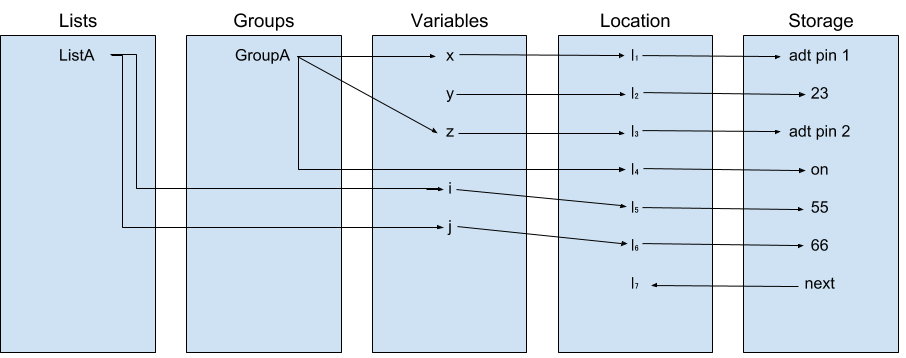
\includegraphics[width=10cm]{figures/semantics/4.png}
  \caption{The model expanded with a list environment}
  \label{fig:listgraphic}
\end{figure}
\noindent
Lists, unlike groups, do not need a location because the list as a whole will not receive a value. A single element in the environment is defined $env_L$. The environment is defined as:
\begin{center}
$EnvL = ListNames \rightharpoonup \mathcal{P}(EnvV) \times \mathcal{P}(EnvG) \times Sto$
\end{center}
Meaning that the list environment is a partial function that maps to the variable environment, group environment or storage the. 
\\\\
Like groups, lists allow all previously declared variables to feature in the declaration. In addition to this, expressions are allowed as elements, meaning the list will point to a value in storage that has to be evaluated through the given expression. This means lists modify the list environment, and the storage in case an expression is present, both through adding the value and moving the next pointer. This gives transitions the shape:
\begin{center}
$\langle D_L,  \: env_L, \: sto\rangle \xrightarrow{}\textsubscript{DL} (env'_L, \: sto')$
\end{center}
The rules for declaration of lists are seen on Rule~\ref{rule:vardcl}.
\begin{equation}\label{rule:listdcl}
\begin{split}
\begin{minipage}{\linewidth}
$[\text{LISTDCL}_\text{BSS}]$
\end{minipage}
\\
\begin{minipage}{\linewidth}
\centering
$\cfrac{\langle D_L,  \: env_L[lx \mapsto \{L_B\}], \: env_L, \: sto \rangle \xrightarrow{}\textsubscript{DL} (env'_L, \: sto')}{\langle\text{list} \: lx \: \{L_B\} \: \textit{new} \: D_L, \: env_L, \: sto \rangle \xrightarrow{}\textsubscript{DL}(env'_L, \: sto')}$
\end{minipage}
\\\\
\begin{minipage}{\linewidth}
\centering
where $env_v, \: sto \vdash \{L_B\} \xrightarrow{}\textsubscript{LB} \: v$
\end{minipage}
\end{split}
\end{equation}
\noindent
The side condition states that all expressions in the body of the list have to be evaluable through the rules established for the body of a list. How the avluation of a constituent \textit{list body} is updated is further elaborated through the rules for the body of the list defined in Appendix~\ref{APP:ListBody}.
\noindent
\subsubsection{Function declarations}
In order to keep track of the necessary information required to execute a function, a procedure environment is introduced. Function declarations update this procedure environment. The transition system is ($\Gamma \textsubscript{Dp}, \xrightarrow{}\textsubscript{Dp}, T \textsubscript{Dp}$), and the configurations are defined as\\
$\Gamma \textsubscript{Dp} = (FuncDcl \times EnvP) \cup EnvP $\\
$T\textsubscript{Dp} = EnvP$
\\
Due to PHAL using static scope rules, transitions take the shape
$env_v, \: env_G, \: env_L \vdash \langle D_P, env_p \rangle \xrightarrow{} \textsubscript{DP} \: env'_P$
\\ 
The other environments are needed to save details about the bindings as part of the information stored about the function \cite{PilenVedTraeetsRod}. Static scope rules mean that only the variable-bindings, group-bindings, list-bindings and procedure-bindings known for a function are those that were in effect when the procedure was declared. Because of this, the procedure-environment needs to remember these bindings, and as such the set $EnvP$ is defined as:
\\\\
$EnvP = Funcnames \rightharpoonup Stmt \times Var \times EnvV \times EnvG \times EnvL \times EnvP $
\\\\
The var component specifies that the formal parameter needs to be remembered.

\begin{equation}\label{rule:funcdclbss}
\begin{split}
\begin{minipage}{\linewidth}
$[\text{FUNCDCL}_\text{BSS}]$
\end{minipage}
\\\\
\begin{minipage}{\linewidth}
\centering
$\cfrac{env_v, \: env_G, \: env_L \vdash \langle D_P, env_p[f \mapsto (S, \: P, \: env_v, \: env_G, \: env_L, \: env_p)]\rangle \xrightarrow{}\textsubscript{DP} \: env'_p}{env_v, \: env_G, \: env_L \vdash \langle \text{define} \: f \: \text{with} \: P \: {F_B} \: \text{returnType} \: RTN \: \textit{newline} D_P, \: env_p\rangle \xrightarrow{}\textsubscript{DP} \: env_p'}$
\end{minipage}
\end{split}
\end{equation}

\noindent
The rule for function declaration can be seen in Rule~\ref{rule:funcdclbss}. In order for function calls to remember the bindings that were in effect during declaration, we explicitly bind the environments to the function $f$ along with the statement to be used and the parameters through $P$. As defined in the syntactic formation in table \ref{tab:syntacticformation}, $P$ can be \textit{none}, one parameter or multiple parameters. The $S$ binding refers to the statements used in the function body $F_B$. 

\subsection*{Function calls}
\begin{equation} \label{EQ:FUNCCALLVALRAP}
\begin{split}
\begin{minipage}{\linewidth}
$[\text{FUNCCALLVAL}_\text{BSS}]$
\end{minipage}
\\\\
\begin{minipage}{\linewidth}
\centering
$\cfrac{env'_v[P \mapsto l_1...l_n] \: env'_G, \: env'_L, \: env'_p \vdash \langle S, sto[l_1...l_n \mapsto v_1...v_n][next \mapsto new \: l], \rangle \xrightarrow{} sto'}{env_v, \: env_G, \: env_L, \: env_p \vdash \langle \text{call} \: f \: \text{with} \: (a_1...a_n), \: sto \rangle \xrightarrow{} sto'}$
\end{minipage}
\\\\
\begin{minipage}{\linewidth}
\centering
where $env_p f = (S, P, env'_v, \: env_G', \: env'_L, \: env'_p),$
\end{minipage}
\\
\begin{minipage}{\linewidth}
\centering
$env_v, \: sto \vdash a_1...a_n \xrightarrow{}\textsubscript{a} \: v_1...v_n$
\end{minipage}
\\
\begin{minipage}{\linewidth}
\centering
$freemem_i = sto[next \mapsto new \: l]$, $l_i = sto \: freemem_i$
\end{minipage}
\\
\begin{minipage}{\linewidth}
\centering
where $1 \leq i \leq n $
\end{minipage}
\end{split}
\end{equation}
\noindent
In call-by-value function calls, the formal parameter appears in the body of the procedure as a local variable. 
This local variable is assigned the value of the actual parameters used for the call. This means that, for each parameter a free memory cell must be found, so that this free memory can contain this local variable, and this variable is initialised with the value of the actual parameter. 
We accomplish this through the side conditions. 
The function is called with $n$ parameters, each one evaluated to a value through the rules for arithmetic expressions. 
After this, the required locations are found through the \textit{free memory (freemem)} variable. 
The store is iterated upon $n$ times, each time finding a new location which is assigned to a location $l$ and the next pointer is updated. 
After this is done, the $n$ found locations are used in the premise of the rule, binding the formal parameters $P$ to their locations. 
As was the case with the FUNCDCL rule (Rule~\ref{rule:funcDcl}), $P$ in this case is either \textit{none}, one parameter or multiple parameters. 
The store is then updated, where the empty locations found are assigned the values evaluated from the actual parameters, creating a correspondence between formal and actual parameters. 
Finally, the next pointer is updated once again, and the store is modified.
\\
\begin{equation} \label{EQ:FUNCCALLRECVALRAP}
\centering
\begin{split}
\begin{minipage}{\linewidth}
$[\text{FUNCCALLRECVAL}_\text{BSS}]$
\end{minipage}
\\
\begin{minipage}{\linewidth}
\centering
$
\dfrac
    {
    \splitdfrac
        {
            env'_v[P \mapsto l_1...l_n], \: env'_G, \: env'_L, \: env'_p[f \mapsto (S, \: P, \: env'_v, \: env'_G, \: env'_L \: env'_p)]
        }
        { 
            \vdash \langle S, sto[l \mapsto v][next \mapsto new \: l] \rangle \xrightarrow{} sto'
        }
    }
    {
        env_v, \: env_G, \: env_L, \: env_p \vdash \langle \text{call} \: f \: \text{with} \: (a_1...a_n), \: sto \rangle \xrightarrow{} sto'
    }
$
\end{minipage}
\\\\
\begin{minipage}{\linewidth}
\centering
where $env_p f = (S, P, env'_v, \: env_G', \: env'_L, \: env'_p),$
\end{minipage}
\\
\begin{minipage}{\linewidth}
\centering
$env_v, \: sto \vdash a_1...a_n \xrightarrow{}\textsubscript{a} \: v_1...v_n$
\end{minipage}
\\
\begin{minipage}{\linewidth}
\centering
$freemem_i = sto[next \mapsto new \: l]$, $l_i = sto \: freemem_i$
\end{minipage}
\\
\begin{minipage}{\linewidth}
\centering
where $1 \leq i \leq n $
\end{minipage}
\end{split}
\end{equation}
\\
This rule is very similar to \ref{EQ:FUNCCALLVALRAP}, but the main difference is found in the procedure-environment used in the premise of the rule. In the previous rule for function calls, $S$ is executed in the procedure-environment $env'_p$, which includes the procedure-bindings known before $f$ was declared. This means that, if we were to execute a second call of $f$ in the statement $s$, the second call in the body would be a different procedure compared to the first call, because $f$ is not declared in $env'_p$ and as such $f$ is not known in that environment. To allow recursive calls, the procedure-environment must then contain a binding of the original function, where the information needed to execute the original function is stored, and the statement $S$ must be executed in the procedure environment that is updated with the binding of $f$. This means we first look up the bindings at the time of declaration, and then create a new environment where these bindings are kept so they can be called recursively.


\subsection*{Statements}
\begin{equation}\label{rule:assignabss}
\begin{minipage}{.2\linewidth}
$[\text{ASSIGNA}_\text{BSS}]$
\end{minipage}
\begin{minipage}{.8\linewidth}
\centering
$env_v \vdash \langle x := a, \: sto \rangle \xrightarrow{} sto[l \mapsto v]$
\\
where $env_v, \: sto \vdash a \xrightarrow{}\textsubscript{a} \: v$ and $env_v \: x = l$
\end{minipage}
\end{equation}
In Rule~\ref{rule:assignabss} the simplest form for statement is seen. It handles binding a variable to an arithmetic expression, \textit{a}. The side condition states that \textit{a} must be evaluated to a value and \textit{x} is a location in the variable environment. Finally the value is mapped to the location in the storage \textit{sto}.


\begin{equation}\label{rule:loopuntiltrue}
\begin{minipage}{.2\linewidth}
$[\text{LOOPUNTIL-TRUE}_\text{BSS}]$
\end{minipage}
\begin{minipage}{.8\linewidth}
\centering
$env_v, \: env_p \vdash \langle $loop $S$ until $b$, sto$\rangle \xrightarrow{} sto$ \\
if $env_v, \: sto \vdash b \xrightarrow{}\textsubscript{b} \: tt$ 
\end{minipage}
\end{equation}
In Rule~\ref{rule:loopuntiltrue}, the boolean expression \textit{b} is evaluated immediately before any iterations of the loop, and as such, if the expression evaluates to true no iteration is conducted. This is evident in the side-condition, where $b$ is evaluated in the original \textit{sto}, rather than the updated store \textit{sto'} which would be created if $b$ were to be evaluated after the iteration of the loop.

\begin{equation}
\begin{split}
\begin{minipage}{\linewidth}
$[\text{LOOPUNTIL-FALSE}_\text{BSS}]$
\end{minipage}
\\\\
\begin{minipage}{\linewidth}
\centering
$\cfrac{env_v \: env_p \vdash \langle S, \: sto \rangle \xrightarrow{} sto'' \quad\: env_v, \: env_p \vdash \langle \text{loop} \: S \: \text{until} \: b, \: sto'' \rangle \xrightarrow{} sto'}{env_v, \: env_p \vdash \langle \text{loop} \: S \: \text{until} \: b, \: sto \rangle \xrightarrow{} sto'}$ 
\end{minipage}
\\\\
\begin{minipage}{\linewidth}
\centering
if $env_v, \: sto \vdash b \xrightarrow{}\textsubscript{b} \: ff$
\end{minipage}
\end{split}
\end{equation}
In order to define the statement that loops S a certain amount of times, we introduce a function that, for any given number, gives the corresponding numeral, the inverse of the function introduced for the arithmetic expressions:
\begin{center}
$\mathcal{N}^{-1}: \mathbb{Z} \xrightarrow{} Num$
\end{center}
This function uses the set of integers, denoted $\mathbb{Z}$, as the number cannot be a floating point number.
\begin{equation}\label{rule:looptimesbss}
\begin{split}
\begin{minipage}{\linewidth}
$[\text{LOOPTIMES}_\text{BSS}]$
\end{minipage}
\\
\begin{minipage}{\linewidth}
\centering
$\cfrac{env_v, \: env_p \vdash \langle S, \: sto \rangle \xrightarrow{} sto'' \: \: \: \: \: \langle \text{loop} \: S \: n \: \text{times}, \: sto'' \rangle \xrightarrow{} sto'}{env_v, \: env_p \vdash \langle \text{loop} \: S \: a \: \text{times} \rangle \xrightarrow{} sto'}$ 
\end{minipage}
\\\\
\begin{minipage}{\linewidth}
\centering
where $env_v, \: sto \vdash a \xrightarrow{} v$
\\
$n = \mathcal{N}^{-1}(v-1)$
\\
$v > 0$
\end{minipage}
\end{split}
\end{equation}
\noindent
The rule~\ref{rule:looptimesbss} states that the loop condition is tested at first in state $s$. This creates a new state $s''$, which is then used for the execution of the actual loop body, finally ending with state $s'$ in both the premise and the conclusion of the rule. The side conditions details when the loop condition is met. The first condition states that the arithmetic expression in state $s$ must be evaluable to a value. The second condition makes use of the function defined above to give the corresponding numeral for the given number based on $v$, where $v$ is decremented for each iteration of the loop. Finally the last condition ensures that the loop is only executed when the value of the arithmetic expression is a positive numeral, this can be seen on rule~\ref{rule:looptimesend}.
\begin{equation}\label{rule:looptimesend}
\begin{minipage}{.2\linewidth}
$[\text{LOOPTIMES-END}_\text{BSS}]$
\end{minipage}
\begin{minipage}{.8\linewidth}
\centering
$env_v, \: env_p \langle \text{loop} \: S \: a \: \text{times}, \: sto \rangle \xrightarrow{} sto$ 
\\
where $env_v, sto \vdash a \xrightarrow{} v \: \text{and} \: v \leq 0$
\end{minipage}
\end{equation}

\subsection*{Switch}
\begin{equation}\label{rule:switchdefault}
\begin{split}
\begin{minipage}{\linewidth}
$[\text{SWITCH-DEFAULT}_\text{BSS}]$
\end{minipage}
\\
\begin{minipage}{\linewidth}
\centering
$\cfrac{env_v, \: env_p \vdash \langle S, \: sto \rangle \xrightarrow{} sto'}{env_v, \: env_p \vdash \langle \text{switch}(e) \{\text{case} <e_1>: \: S_1  \: \text{default:} \: S\}, \: sto \rangle \xrightarrow{} sto' }$ 
\end{minipage}
\\\\
\begin{minipage}{\linewidth}
\centering
where $env_v, \: env_p \vdash e \xrightarrow{} v$
\\
$env_v, \: env_p \vdash e_1 \xrightarrow{} v_1$
\\
$v \neq v_1$
\end{minipage}
\end{split}
\end{equation}
Rule \ref{rule:switchdefault} defines the case where $n=1$, meaning there is only one switch case followed by the default case. In this case, if the expression being switched can evaluate to a value, and the expression of the first case can evaluate to a value, but these values are not similar, the switch will execute the default statement $S$ in state $s$.
\begin{equation}\label{rule:switch1bss}
\begin{split}
\begin{minipage}{\linewidth}
$[\text{SWITCH-1}_\text{BSS}]$
\end{minipage}
\\
\begin{minipage}{\linewidth}
\centering
$\cfrac
{
    env_v, \: env_p \vdash \langle S_1, \: sto \rangle \xrightarrow{} sto'
}
{
   env_v, \: env_p \vdash \langle \text{switch}(e) \{\text{case} <e_1>: \: S_1 ... \text{case} <e_n>: \: S_n \: \text{default:} \: S\}, \: sto \rangle \xrightarrow{} sto' 
}
$ 
\end{minipage}
\\\\
\begin{minipage}{\linewidth}
\centering
if $ n \geq 1$ and $env_v, \: env_p \vdash e \xrightarrow{} v$
\\
$env_v, \: env_p \vdash e_1 \xrightarrow{} v_1$
\\
$v = v_1$
\end{minipage}
\end{split}
\end{equation}
The Rule~\ref{rule:switch1bss} accounts for the possibility where $n$ is greater than or equal to $1$, meaning it is possible to have multiple cases not including the default case, but the value of $e$ is evaluated to the value of $e_1$, making the first case the one to be executed. In the case where $ n = 1$, meaning there is only one case and the default, this rule serves as the opposite of the SWITCH-DEFAULT rule, executing the first case.
\begin{equation}\label{rule:switch2bss}
\begin{split}
\begin{minipage}{\linewidth}
$[\text{SWITCH-2}_\text{BSS}]$
\end{minipage}
\\
\begin{minipage}{\linewidth}
\centering
$\cfrac
{
    env_v, \: env_p \vdash \langle  \text{switch}(e) \{\text{case} <e_2>: \: S_2 ... \text{case} <e_n>: \: S_n \: \text{default:} \: S\}, \: sto \rangle \xrightarrow{} sto'
}
{
    env_v, \: env_p \vdash \langle \text{switch}(e) \{\text{case} <e_1>: \: S_1 ... \text{case} <e_n>: \: S_n \: \text{default:} \: S\}, \: sto \rangle \xrightarrow{} sto' 
}$ 
\end{minipage}
\\\\
\begin{minipage}{\linewidth}
\centering
if $ n > 1$ and $env_v, \: env_p \vdash e \xrightarrow{} v$
\\
$env_v, \: env_p \vdash e_1 \xrightarrow{} v_1$
\\
$v \neq v_1$
\end{minipage}
\end{split}
\end{equation}
The Rule~\ref{rule:switch2bss} deals with the possibility of having multiple cases, meaning that $n$ is strictly greater than 1, and the first case not matching the value evaluated. In this case, the premise removes the first option that was evaluated to false, and the next expression in line is evaluated according to $e$. This rule interacts with SWITCH-1 (Rule~\ref{rule:switch1bss}), as they in unison serve to find the correct case. If $n$ reaches $1$, and this is once again evaluated to be different than the original expression, the SWITCH-DEFAULT rule (Rule~\ref{rule:switchdefault}) ensures that the switch is terminated properly.

\subsubsection{If-else}

\begin{equation}\label{sem:IfNoElseTT}
\begin{minipage}{.2\linewidth}
$[\text{IFNOELSE-TRUE}_\text{BSS}]$
\end{minipage}
\begin{minipage}{.8\linewidth}
\centering
$\cfrac{env_v, \: env_p \vdash \langle S, \: sto\rangle \xrightarrow{} sto'}{env_v, \: env_p \vdash \langle \text{if} \: b \: \text{then} \: S, \: sto \rangle \xrightarrow{} sto'}$ 
\\
if $env_v, \: sto \vdash b \xrightarrow{}\textsubscript{b} \: tt$
\end{minipage}
\end{equation}
The Rule~\ref{sem:IfNoElseTT} deals with the simplest case of an if-statement, where there is no following else statement. In this case, if the expression is evaluated to true, the statement $S$ is executed and the storage is updated.\\
In the opposite case, where the expression evaluates to false, there will be no further consequences of the rule. The rule for this can be found on Rule~\ref{listing:ifnoelse-false}.
\\
If-statements can chain together multiple \textit{else-if} clauses. In order to facilitate this, the syntactic category $S_{if}$ is introduced. In this category, three possibilities for ending if-statements are detailed. The two following rules deal with the if-statements found in the S category that contain the $S_{if}$ category.
\begin{equation}\label{rule:ifelsetrue}
\begin{minipage}{.2\linewidth}
$[\text{IFELSE-TRUE}_\text{BSS}]$
\end{minipage}
\begin{minipage}{.8\linewidth}
\centering
$\cfrac{env_v, \: env_p \vdash \langle S, \: sto \rangle \xrightarrow{} sto'}{env_v, \: env_p \vdash \langle \text{if} \: b \: \text{then} \: S \:S_{if}, \: sto \rangle \xrightarrow{} sto'}$ 
\\
if $env_v, \: sto \vdash b \xrightarrow{}\textsubscript{b} \: tt$
\end{minipage}
\end{equation}
The Rule~\ref{rule:ifelsetrue} is similar to the one detailing if-structures without else clauses seen in Rule~\ref{sem:IfNoElseTT}. The only difference is in the conclusion, in the way the if-structure is detailed. For this rule, the use of an else clause is allowed, but specifies that the condition for the \textit{if} is evaluated to true, and as such, the statement $S$ related to the \textit{if} is executed.
\\\\
The case where the boolean expression $b$ evaluates to false requires the use of the $s_{if}$ category, and the rules for this category will be detailed in the following section.
\textbf{The $S_{if}$ category}\\
The Rules~\ref{rule:elseifseqtrue} and \ref{rule:elseifseqtrue} detail the possible endings to if-statements in PHAL.

\begin{equation}\label{rule:elseifseqtrue}
\begin{minipage}{.2\linewidth}
$[\text{ELSEIFSEQ-TRUE}_\text{BSS}]$
\end{minipage}
\begin{minipage}{.8\linewidth}
\centering
$\cfrac{env_v, \: env_p \vdash \langle S, \: sto \rangle \xrightarrow{} sto'}{env_v, \: env_p \vdash \langle \text{else if} \: b \: \text{then} \: S \: S_{if}, \: sto \rangle \xrightarrow{} sto'}$ 
\\
if $env_v, \: sto \vdash b \xrightarrow{}\textsubscript{b} \: tt$
\end{minipage}
\end{equation}
This rule describes the case where there's an \textit{else-if} statement following an \textit{if}, and the \textit{else-if} evaluates to true.\\
In this case, the statement $S$ bound to the \textit{else-if} clause is executed and the storage is updated.

\begin{equation}\label{rule:elseend}
\begin{minipage}{.2\linewidth}
$[\text{ELSEEND}_\text{BSS}]$
\end{minipage}
\begin{minipage}{.8\linewidth}
\centering
$\cfrac{env_v, \: env_p \vdash \langle S, \: sto \rangle \xrightarrow{} sto'}{env_v, \: env_p \vdash \langle \text{else} \: S, \: sto \rangle \xrightarrow{} sto'}$ 
\end{minipage}
\end{equation}
Rule~\ref{rule:elseend} defines the case where an \textit{else} clause is defined in the \textit{if}-structure, and all the previous cases evaluated to false. In this case, this means that the statement $S$ bound to the \textit{else}-clause is executed by default, updating the storage.

\section{Type rules}\label{subsec:FormalTypeRules}
In order to precisely define the type rules we create a type system for PHAL. The type system is used to define a classification for the syntactic entities of a program. This is used as a guarantee to prevent the runtime errors that the type system aims to prevent.  A simple example of why type system are useful can be found in the following expression that is allowed in PHAL:
\begin{center}
$12 + (12 > 14)$
\end{center}
This expression attempts to add a boolean expression and a numeral that evaluates to the PHAL type \textit{number}. This would lead to a runtime error. This can be avoided by giving both components of the expression a type, and requiring in an addition expression that both components need to be of the type \textit{number} to avoid errors. For PHAL, the types used in the type system are the same as the ones defined in Section~\ref{Def:Types} - \textit{bool, number, text, group and list}. A type system consists of:
\begin{itemize}
    \item A definition of the set of types
    \item A definition of the type judgement for the elements of each syntactic category in the language
    \item A number of type rules for each category that define the valid type judgement\cite{PilenVedTraeetsRod}
\end{itemize}

\subsubsection{Operator precedence-table}
In addition to the type rules, the precedence and associativity of the operators must be specified. The precedence of operators ensures that the operator grammar is unambiguous. 
It was chosen to use a precedence that imitates the operator precedence that is used in mathematics. This is done to ensure that the arithmetic operations and logical operations in PHAL are as intuitive as possible for the user. 

\begin{table}[H]
\centering
\caption{Operator precedence for PHAL}
\label{tab:operatorprecedence}
\begin{tabular}{|l|l|l|l|}
\hline
\textbf{Precedence} & \textbf{Operator}                                                                                                                                                                       & \textbf{Description}                                                                                                                                                                             & \textbf{Associativity} \\ \hline
1                   & ( )                                                                                                                                                                                     & Subexpression                                                                                                                                                                                    & Left to right          \\ \hline
2                   & \begin{tabular}[c]{@{}l@{}}!\\ not\end{tabular}                                                                                                                                         & \begin{tabular}[c]{@{}l@{}}Logical negation\\ Logical negation\end{tabular}                                                                                                                      & Left to right          \\ \hline
3                   & \begin{tabular}[c]{@{}l@{}}*\\ /\end{tabular}                                                                                                                                           & \begin{tabular}[c]{@{}l@{}}Multiplication\\ Division\end{tabular}                                                                                                                                & Left to right          \\ \hline
4                   & \begin{tabular}[c]{@{}l@{}}+\\ -\end{tabular}                                                                                                                                           & \begin{tabular}[c]{@{}l@{}}Plus or concatenation\\ Minus\end{tabular}                                                                                                                            & Right to left          \\ \hline
5                   & \begin{tabular}[c]{@{}l@{}}\textless\\ is less than\\ \textless=\\ is less than or equal to\\ \textgreater\\ is greater than\\ \textgreater=\\ is greater than or equal to\end{tabular} & \begin{tabular}[c]{@{}l@{}}Less than\\ Less han\\ Less than or equal to\\ Less than or equal to\\ Greater than\\ Greater than\\ Greater than or equal to\\ Greater than or equal to\end{tabular} & Left to right          \\ \hline
6                   & \begin{tabular}[c]{@{}l@{}}=\\ is\\ !=\\ is not\end{tabular}                                                                                                                            & \begin{tabular}[c]{@{}l@{}}Equality comparison\\ Equality comparison\\ Inequality comparison\\ Inequality comparison\end{tabular}                                                                & Left to right          \\ \hline
7                   & \begin{tabular}[c]{@{}l@{}}\&\\ and\end{tabular}                                                                                                                                        & \begin{tabular}[c]{@{}l@{}}Logical and\\ Logical and\end{tabular}                                                                                                                                & Left to right          \\ \hline
8                   & \begin{tabular}[c]{@{}l@{}}or\\ ||\end{tabular}                                                                                                                                         & \begin{tabular}[c]{@{}l@{}}Logical or\\ Logical or\end{tabular}                                                                                                                                  & Left to right          \\ \hline
9                   & :=                                                                                                                                                                                      & Assignment                                                                                                                                                                                       & Right to left          \\ \hline
\end{tabular}
\end{table}

\noindent
\subsubsection*{Changes to the abstract syntax}
When creating the rules for the semantics of PHAL, we defined an abstract syntax as shown in Table~\ref{tab:syntacticcategories}, Section~\ref{Def:Semantics}. To create the type system, this syntax is modified to include type for declarations of the different categories of variables. To do this, we use the metavariable $T$ to define an element of the category of types defined as \textit{Types}. 
\begin{table}[H]
\centering
\begin{tabular}{@{}lll@{}}
\toprule
Variable &       & Description                      \\ \midrule
$e$       & $::=$ &  $n$ | $x$ | $gx$ | $lx$ | $e_1 + e_2$ | $e_1 - e_2$ | $e_1 * e_2$ | $e_1 \div e_2$ | $e_1 \bmod e_2$ | $ (e_1)  $ \\
          && | $e_1 = e_2$ | $e_1 != e_2$ | $e_1 > e_2$ | $e_1 >= e_2$            \\
            & & | $!e$ | $e_1$ \& $e_2$ | $e_1 | e_2$ \\
            &&  | $e_1$ is $e_2$ | $e_1$ and $e_2$  | $e_1$ or $e_2$ |  $e_1$ is not $e_2$ | not $e$ \\
            &&  | $e_1$ greater than $e_2$  |  $e_1$ less than $e_2$  | $e_1$ less than or equal to $e_2$ \\
            &&  | $e_1$ greater than or equal to $e_2$ \\
            & & | true | false | on | off \\
$S$        & $::=$ & $x:= e$ | $gx := e$ | $S_1 \textit{new} \: S_2$ | if ($e$) then \{$S$\} $S_{if}$ | if ($e$) then \{$S$\} \\
           & & | loop $S$ until $e$ | loop $S$ until $e$, increase x by n    \\
           & & | loop $S$ until $e$, decrease $x$ by $n$ | loop $S$ $e$ times \\
           & & | call $f$ with ($e...e_n$)  \\
           & & | switch($e$) \{case $<e_1>: \: S_1$ $...$ case $<e_n>: \: S_n$ default: $S$ \} \\
           &&  | get element $n$ from $lx$ | remove element $n$ from $lx$  \\
           &&  | add $e$ to $lx$ |  $\text{wait for } e \text{ seconds}$  \\
$S_{if}$     & $::=$ &  else if ($e$) then \{$S$\} | else if ($e$) then \{$S$\} $S_{if}$ |  else \{$S$\} \\
$D_V$       & $::=$ & $T \: var$ $x := e \: \textit{new}$ $D_V$ | $\epsilon$ \\
$D_G$       & $::=$ & $T \: var \: gx\{ G_B \} \: \textit{new} \: D_G | \: \epsilon$ \\
$D_L$     & $::=$ &  $T \: var \: lx\{ L_B \} \: \textit{new} \: D_L | \: \epsilon$ \\
$D_F$       & $::=$ & define $f$ with ($T \: P$) \{$F_B\} \: \text{returnType} \: (RTN) \: \textit{new}$ $D_F$ | $\epsilon$ \\
$D_P$  & $::=$ &  $T \: x, \: D_P \: | \: T \: x $  \\
$D_{Adt}$   & $::=$ & $T \: var$ $x$ $:=$ pin $Pin \: new \: D_{adt} | \: \epsilon  $\\
\bottomrule
\end{tabular}
\caption{Syntactic formation of PHAL updated for the type system}
\label{tab:syntacticformationtypes}
\end{table}
\noindent
Table~\ref{tab:syntacticformationtypes} has removed the metavariables $a$ and $b$ used for defining the semantics of PHAL, and swapped all occurrences of these with the metavariable $e$, to denote a generalised expressions. This also means that the occurrences of $a$ or $b$ in the statement elements have been swapped to $e$. Because of this change, we update the previous table of syntactic categories shown on Table~\ref{tab:syntacticcategories}to reflect the introduction of $e$:
\begin{table}[H]
\centering
\begin{tabular}{@{}lll@{}}
\toprule
Variable &       & Description                      \\ \midrule
$n$        & $\in$ & \textbf{Num} - Number                     \\
$x$        & $\in$ & \textbf{Var} - Variable                     \\
$gx$        & $\in$ & \textbf{GVar} - A variable of the group type                     \\
$lx$        & $\in$ & \textbf{LVar} - A variable of the list type                     \\
$\epsilon$ & $\in$ & \textbf{Epsilon} - The empty string \\
$new$      & $\in$ &  \textbf{Newl} - Newline                   \\
$e$        & $\in$ & \textbf{Exp} - The combined category for arithmetic and boolean expressions                \\
$adt$        & $\in$ & \textbf{Adv} - Advanced data type                     \\
$f$       & $\in$ & \textbf{FuncName} - The name of a function      \\
$S$        & $\in$ & \textbf{Stmt} - Statements               \\
$D_V$       & $\in$ & \textbf{VarDcl} - Declaration of a variable \\
$D_G$       & $\in$ & \textbf{GroupDcl} - Declaration of a group \\
$D_L$       & $\in$ & \textbf{ListDcl} - Declaration of a list \\
$D_F$       & $\in$ & \textbf{FuncDcl} - Declaration of a function \\
$D_{Adt}$       & $\in$ & \textbf{AdvDcl} - Declaration of an advanced type      \\
$D_P$       & $\in$ & \textbf{ParamDcl} - Declaration of parameters for a function \\
$P$       & $\in$ & \textbf{ParamOpt} - The parameter options \\
$Pin$      & $\in$ &  \textbf{Pins} - The pins that are used to connect the Arduino \\
$RTN$       & $\in$ & \textbf{Rtrn} - The returntypes \\
$P_S$        & $\in$ & \textbf{ProgStart} - The start of the program \\
$S_B$       & $\in$ & \textbf{SetBody} - The construction of setup      \\
$G_B$       & $\in$ & \textbf{GrpBody} - The body of the group \\
$L_B$       & $\in$ & \textbf{ListBody} - The body of the list \\
$L_T$       & $\in$ & \textbf{ListType} - The type of the list \\
$F_B$      & $\in$ &  \textbf{FuncBody} - The user defined function body  \\ 
$F_N$      & $\in$ &  \textbf{FuncNames} - The function names  \\
$L_N$      & $\in$ &  \textbf{ListNames} - The list names  \\
$G_N$      & $\in$ &  \textbf{GrpNames} - The group names  \\\bottomrule
\end{tabular}
\caption{Syntactic categories of PHAL}
\label{tab:updatedsyntacticcategories}
\end{table}
\noindent 
We can now define a new transition system for expressions that includes both of the previous definitions:

\begin{equation*}
(\textbf{Exp} \cup \; \mathbb{Q} \cup \; \{tt, \; ff\}, \: \xrightarrow{}\textsubscript{e}, \: \mathbb{Q} \cup \; \{tt, \; ff\})    
\end{equation*}
The transition relation $\xrightarrow{}\textsubscript{e}$ is defined by the updated list of rules given for expressions in Appendix~\ref{typerules:TypeRules}, Section~\ref{typerules:UpdatedExpressions}.

\subsubsection{The types in the type system}
The type system contains the following types:
\begin{equation}
\begin{split}
\text{B} &::= \text{number } | \text{ text } | \text{ bool } | \text{ group } | \text{ list } | \text{ motor } | \text{ temperatureSensor } | \text{ lightbulb}
\\
\text{G} &::= \text{ motor } | \text{ temperatureSensor } | \text{ lightbulb}
\\
\text{T} &::= \text{B } | \text{ G } |  \: x_1...x_n  : B_1...B_n \xrightarrow{} \text{ok } | \text{ ok}
\end{split}
\label{typerules:basistypes}
\end{equation}
The category of types is named $Types$, and elements of this category are denoted with the metavarabile $T$. The concrete types of PHAL are represented as a subset of all types T, denoted by the metavariable $B$ for basic types. Because groups are limited in which types they can contain, a category for the valid group types is also defined as a subset of $T$, denoted $G$.
The type of a function will be the composite type $x_1...x_n : B_1...B_n \xrightarrow{} \text{ok}$, which states that if the types of the formal parameters of the function are $B$, then the statement executing the functions body will be well-typed \cite{PilenVedTraeetsRod}. We also add the type \textit{ok}, which is the type of statements, declarations and functions if they do not have any type errors. These types are shown as part of the category for all types $T$ on Equation~\ref{typerules:basistypes}. 



\subsubsection{Type environments}
To keep track of the type of any given variable we introduce a type environment. This type environment is defined as the partial function:
\begin{align}\label{TypeRules:EDefinition}
    \text{E} : \text{Var} \cup \text{FuncNames} \rightharpoonup \text{Types}
\end{align}
We also need to be able to update type-environments. We let $E$ be a type environment, and let $E[x \mapsto T]$ describe the type environment $E'$ defined by:
\\\\
\begin{equation*}
    E'(y)=
    \begin{cases}
    E(y) \;\; &\text{if} \; y \neq x\\
    T \;\;    &\text{if} \; y = x
    \end{cases}
\end{equation*}
\\\\
This definition states that we want to update the environment $E$ by mapping the variable $x$ to the type $T$ in the environment. We do this by looking through the current environment $E$ searching for the variable we want to update, denoted by $y$. This is written as $E(y)$. If we find a variable $x$ matching the $y$ variable, we know that the correct variable exists in the environment, and we update it with type $T$, resulting in the updated environment $E'(y)$. If no matching variable is found, it does not exists in the environment an error occurred and no change can be made.
\\\\
\textbf{The format of type judgements}
\\\\
The \textit{type judgements} tell us the  following, where the environment $E$ is defined as in Equation~\ref{TypeRules:EDefinition}:
\\\\
$E \vdash e : T$ - an expression has a type $T$
\\\\
$E \vdash D_v : \text{ok}$ - variable declarations have the type \textit{ok}
\\\\
$E \vdash D_f : \text{ok}$ - function declarations have the type \textit{ok}
\\\\
$E \vdash D_G : \text{ok}$ - group declarations have the type \textit{ok}
\\\\
$E \vdash D_L : \text{ok}$ - list declarations have the type \textit{ok}
\\\\
$E \vdash S : \text{ok}$ - statements declarations have the type \textit{ok}
\\\\
$E \vdash S_{if} : \text{ok}$ - if-statement-ending have the type \textit{ok}
\\\\
$E \vdash Pin : Number$ - pins are required to be of the type \textit{number}
\\\\
Because these different categories can include variables, the type-environment $E$ is included as a prerequisite for the type judgements. In the following section we will describe the rules that detail how you assign types to the syntactic elements for some chosen categories. The remaining rules can be found in Appendix~\ref{app:typerulesforvalid}.
\\\\
\textbf{Type rules for valid type judgements for expressions}
\begin{equation}\label{eq:addnum}
\begin{minipage}{.2\linewidth}
$[\text{ADDNUM}_\text{EXP}]$ 
\end{minipage}
\begin{minipage}{.8\linewidth}
\centering
$\cfrac{E \vdash e_1 : \text{Number } \: \: E \vdash e_2 : \text{Number}}{E \vdash e_1 + e_2 : \text{Number}}$
\end{minipage}
\end{equation}
\begin{equation}\label{eq:addtext}
\begin{minipage}{.2\linewidth}
$[\text{ADDTEXT}_\text{EXP}]$ 
\end{minipage}
\begin{minipage}{.8\linewidth}
\centering
$\cfrac{E \vdash e_1 : \text{Text } \: \: E \vdash e_2 : \text{Text}}{E \vdash e_1 \circ e_2 : \text{Text}}$
\end{minipage}
\end{equation}
\noindent
The \textit{add} rule has been split into two, to accommodate the operator overloading. In Listing~\ref{eq:addnum} the rule for adding two numbers is seen. 
It requires the expressions $e_1$ and $e_2$ to both evaluate to a \textit{Number}, in this case the numeric value of the two can be added together using the mathematical addition rule.
\\\\
Likewise, if $e_1$ and $e_2$ are of type \textit{Text}, the rule for adding two \textit{Text} types can be used. 
This rule can be seen on Listing~\ref{eq:addtext}. 
The main difference being that instead of using the mathematical addition rule, they are concatenated. 




\begin{equation}
\begin{minipage}{.2\linewidth}
$[\text{VAR}_\text{EXP}]$
\end{minipage}
\begin{minipage}{.8\linewidth}
\centering
$\cfrac{E(x) = T} {E \vdash x : T}$
\end{minipage}
\end{equation}
This rule simply states that we look for $x$ in the environment $E$ through the $E(x)$ notation, and this returns the type of $x$.

\begin{equation}\label{TypeRules:GrpVar}
\begin{minipage}{.2\linewidth}
$[\text{GRPVAR}_\text{EXP}]$
\end{minipage}
\begin{minipage}{.8\linewidth}
\centering
$\cfrac{E[gx \mapsto (x_1...x_n : G_1...G_n)] \vdash E(gx) = \text{ok} } {E \vdash gx : \text{ok}}$
\end{minipage}
\end{equation}
Groups can only contain a certain set of types, therefore it is needed to check if each element can be evaluated to type $G$, meaning that they are correctly defined. If this is the case, the type of the group variable when looked up in environment $E$ will be $ok$, as groups in PHAL do not have a specific type by themselves, but ensure a combination of different types can be used by the programmer.


\begin{equation}
\begin{minipage}{.2\linewidth}
$[\text{LISTVAR}_\text{EXP}]$
\end{minipage}
\begin{minipage}{.8\linewidth}
\centering
$\cfrac{E[lx \mapsto (gx_1...gx_n : ok,\: x_1...x_n : T \xrightarrow{} ok)] \vdash E(lx) = T } {E \vdash lx : T}$
\end{minipage}
\end{equation}
Lists can contain groups and variables. This means the environment $E$ has to be updated with the bindings of the components of the list. If the group variables can be evaluated to type $ok$, it means that the constituent variables of each group are correctly typed as defined in the rule for type checking groups, Rule~\ref{TypeRules:GrpVar}. On top of this, the bindings for the separate variables in the list must be correctly typed as type $T$. If the conditions are met, the list variable $lx$ can be looked up in the environment and typed as $T$. 

\subsubsection{Type rules for declarations}
To construct the type rules for declarations we need to define certain helper functions. These functions need to return the updated type-environment given by a declaration, when we know the type-bindings for the environment $E$ prior to the declaration. The functions are defined as such:
\begin{equation}\label{typehelp1}
    E(\epsilon, \: E) = E
\end{equation}

\begin{equation}\label{typehelp2}
    E(T \: var \: x := e \: new \: D_V, \: E) = E(D_V, \: E[x \mapsto T])
\end{equation}

\begin{equation}\label{typehelpADT}
    E(T \: var \: x := \text{pin} \: Pin \: new \: D_{adt}, \: E) = E(D_{adt}, \: E[x \mapsto T])
\end{equation}

\begin{equation}\label{typehelp3}
    E(T \: var \: gx := \{G_B\} \: new \: D_G, \: E) = E(D_G, \: E[gx \mapsto (x_1...x_n : T_1...T_n)\xrightarrow{}ok])
\end{equation}

\begin{equation}\label{typehelp4}
    E(T \ var \ lx \: := \: \{L_B\} \: new \: D_L, \: E) = E(D_L, \: E[lx \mapsto (gx_1...gx_n : T_1...T_n \xrightarrow{} ok, \: x_1...x_n : T_1...T_n \xrightarrow{} ok)])
\end{equation}

 \begin{equation} \label{typehelp5}
     E(\text{define} \, f \, \text{with} \, (T \, P) \, \{F_B\} \, \text{returnType} \, (RTN) \, new \, D_F, \, E) = E(D_F, \, E[f \mapsto (P:T_1...T_n) \xrightarrow{}\text{ok}])
 \end{equation}
\\
These functions define the resulting type environment after declarations. In the case of function \ref{typehelp1}, it states that updating type-environment $E$ with $\epsilon$ is equivalent to an environment that is unchanged as it is an empty declaration. Function \ref{typehelp2} concerns declarations of variables. It states that when the environment $E$ is updated with a variable declaration, the updated type-environment is one where the variable $x$ defined in the declaration is mapped to the type $T$. The next function, Function~\ref{typehelpADT} is similar to Function~\ref{typehelp2}.
\\\\
Function \ref{typehelp3} describes the updated environment after a group has been declared. The environment $E$ is updated to contain a variable $gx$, of type ok if all of the $n$ elements contained in the group can evaluate to a type $T$. The next function, Function~\ref{typehelp4}, is for list variables. It updates the environment $E$ with the variable $lx$ if all the group variables declared in it are of type $T$ and all regular variables are of the same type, $T$.
\\\\
Function \ref{typehelp5} states that when a function is declared, the resulting type-environment is one where the function $f$ has the type $(x_1...x_n : T_1...t_n)$, meaning the parameters are valid and the declaration is \textit{ok}.
\begin{equation}\label{rule:vardcll}
\begin{minipage}{.2\linewidth}
$[\text{VAR}_\text{DCL}]$
\end{minipage}
\begin{minipage}{.8\linewidth}
\centering
$\cfrac{E \vdash e : T \: \: \: \: E[x \mapsto T] \vdash D_V : \text{ok}} {E \vdash T \: var \: x := e \: new \: D_V : \text{ok}}$
\end{minipage}
\end{equation}
Rule~\ref{rule:vardcll} states that, if you have a variable declaration, $e$ needs to be type checked first, and then the remaining declarations are type checked in an environment where variable $x$ is of type $T$, because that variable might appear in other declarations. 

\begin{equation}\label{rule:adtdcl}
\begin{minipage}{.2\linewidth}
$[\text{ADT}_\text{DCL}]$
\end{minipage}
\begin{minipage}{.8\linewidth}
\centering
$\cfrac{E \vdash pin : T \: \: \: \: E \vdash Pin : ok \: \:  \: \: E[x \mapsto T] \vdash D_{adt} : \text{ok}} {E \vdash T \: var \: x := \text{pin} \: Pin \: new \: D_{adt} : \text{ok}}$
\end{minipage}
\end{equation}
The rule~\ref{rule:adtdcl} is similar to variables but differs in that it requires the category \textit{Pin}. As such, the type rule for \textit{Pin} are shown as a helper rule below. In order to type check an advanced data type, the type of the pin must be checked as $T$, the \textit{Pin} category must be checked to be \textit{ok}, and then the remaining declarations can be checked in an environment updated with the variable $x$ bound to type $T$.

\begin{equation}\label{pinhlpr}
\begin{minipage}{.2\linewidth}
$[\text{PIN}_\text{HLPR}]$
\end{minipage}
\begin{minipage}{.8\linewidth}
\centering
$\cfrac{E \vdash n_1, \dots n_n : Number} {E \vdash n_1, \dots n_n : \text{ok}}$
\end{minipage}
\end{equation}
The rule~\ref{pinhlpr} simply states that for the \textit{Pin} category to be correct all elements must be of type \textit{Number}. 

\begin{equation}\label{rule:funcDcl}
\begin{minipage}{.2\linewidth}
$[\text{FUNC}_\text{DCL}]$
\end{minipage}
\begin{minipage}{.8\linewidth}
\centering
$\cfrac{E[P : T_1...T_n] \vdash S : \text{ok} \: \: \: E[f \mapsto (P: T_1...T_n \xrightarrow{} ok)] \vdash D_P : \text{ok}}{E \vdash \text{define} \: f \: \text{with} \: (T \: P) \{F_B\} \: \text{returnType} \: (RTN) \: \textit{new} \: D_F : \text{ok}}$
\end{minipage}
\end{equation}
\\
The rule~\ref{rule:funcDcl} defines declarations of functions. The first declaration is type checked by type checking the body $S$ of the function, where the formal parameters are assumed to be correctly typed. After this has been type checked, the assumption that function $f$ receives something of type $T$ and returns an $ok$ command can be used to check remaining declarations by expanding the environment $E$.
\\\\
\textbf{Type rules for statements}
\\\\
The type judgement for statements is $E \vdash S : \text{ok}$,  meaning that certain runtime errors cannot appear anywhere in the statement $S$.
\\
\begin{equation}\label{rule:if1stm}
\begin{minipage}{.2\linewidth}
$[\text{IF-1}_\text{STM}]$
\end{minipage}
\begin{minipage}{.8\linewidth}
\centering
$\cfrac{E \vdash e : \text{Bool } \text{ E} \vdash S : \text{ok }}{E \vdash \text{if } e \text{ then } S : \text{ok}}$
\end{minipage}
\end{equation}
Typechecking for if statements is quite simple, as seen on Rule~\ref{rule:if1stm}. First the expression is checked, in order for it to be evaluated upon, it must be of type \textit{Bool}. Likewise, the body (\textit{S}) of the if statement must be type ok. Given these conditions, the if statement is type ok.


\begin{equation}\label{rule:addlistelestmt}
\begin{minipage}{.2\linewidth}
$[\text{ADDLISTELE}_\text{STM}]$
\end{minipage}
\begin{minipage}{.8\linewidth}
\centering
$\cfrac{E \vdash e : T \: \: \: E[lx \mapsto \text{List}] \: lx : T} {E \vdash \text{add } e \text{ to } lx: \text{ok} }$
\end{minipage}
\end{equation}
To add an element to a list, which is described in Rule~\ref{rule:addlistelestmt}, it must first be checked whether the expression is typed as type T. In addition to this, the list must also be typed as type T. If these are true, the addition to the list is type correct.

\begin{equation}\label{rule:callsmt}
\begin{minipage}{.2\linewidth}
$[\text{CALL}_\text{STM}]$
\end{minipage}
\begin{minipage}{.8\linewidth}
\centering
$\cfrac{E \vdash f : (P_1...P_n : T_1...T_n \xrightarrow{}\text{ok}) \: \: \: E \vdash e : T}{E \vdash \text{call} \: f \: \text{with} \: (e_1...e_n) : \text{ok}}$
\end{minipage}
\end{equation}
To typecheck a function call, the function $f$ is looked up in the type environment, as seen on Rule~\ref{rule:callsmt}, and $f$ is then typed as $(P_1...P_n : T...T_n \xrightarrow{} ok)$. After this, the actual parameters $e_1...e_n$ are typed as type $T$. The type check of the functions body is done during declaration, and the declaration told us that the function is ok if it is given a parameter of type $T$.